\documentclass{article}
\usepackage{graphicx}
\usepackage{amsmath}

\usepackage{listings}
\usepackage{color}

\definecolor{backcolour}{rgb}{0.95,0.95,0.92}

\lstdefinestyle{mystyle}{
    backgroundcolor=\color{backcolour}
    }

\lstset{style=mystyle}

\title{Statistical Modeling 2 \\ Exercise 3}

\begin{document}
\maketitle
\section*{Basic concepts}
\begin{align*}
\mbox{MSE}(\hat{f}, f) &= E\{[f(x) - \hat{f}(x)]^2\}\\
&= E [ f(x)^2 + \hat{f}(x)^2 - 2f(x)\hat{f}(x)]\\
&=  f(x)^2 + E[\hat{f}(x)^2] - E[\hat{f}(x)]^2 + E[\hat{f}(x)]^2 - 2 f(x) E[\hat{f}(x)]\\
&= \{E[\hat{f}(x)^2] - E[\hat{f}(x)]^2\} + \{f(x)^2 + E[\hat{f}(x)]^2 - 2 f(x) E[\hat{f}(x)]\}\\
&= V + B^2
\end{align*}


\section*{Curve fitting by linear smoothing}
\subsection*{A}
In the least square estimate, we minimize:
\begin{align*}
L = \sum_{i=1}^n (\hat{\beta}x_i - y_i)^2
\end{align*}
We take the derivative and set to \(0\):
\begin{align*}
\partial L / \partial \hat{\beta} &= \sum_{i=1}^n 2 (\hat{\beta}x_i - y_i) x_i = 0\\
&\implies \hat{\beta}(\sum_{i=1}^n x_i^2) - \sum_{i=1}^n y_i x_i = 0\\
&\implies \hat{\beta} = \frac{\sum_{i=1}^n y_i x_i}{ \sum_{i=1}^n x_i^2}
\end{align*}
We have that the prediction is:
\begin{align*}
\hat{f}(x^*) &= \hat{\beta} x^*\\
&= \frac{\sum_{i=1}^n x_i x^* y_i}{ \sum_{i=1}^n x_i^2}\\
&= \sum_{i=1}^n w(x_i, x^*) y_i 
\end{align*}
where
\begin{align*}
w(x_i, x^*) = \frac{x_i x^*}{ \sum_{i=1}^n x_i^2}
\end{align*}

This weight function weights examples by the product with predictors, using all the points in the dataset. The K nearest function weights the \(K\) nearest neighbors equally and ignore all other points. 

\subsection*{B}
Code: kernel.r

\noindent
I use the function \textsf{sin} from $-5$ to $5$ with $100$ samples and try three bandwidths: \(h = 0.01, h = 0.1, h = 1\).

\begin{figure}[h!]
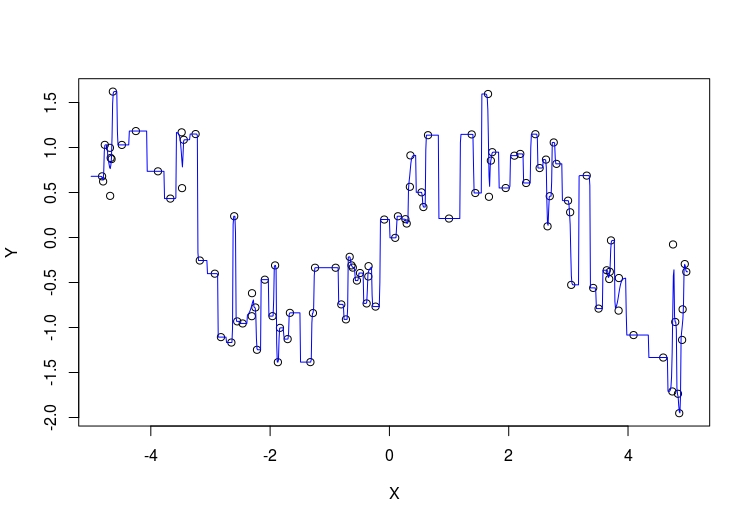
\includegraphics[width = \textwidth]{h001.jpeg}
\caption{Bandwidth \(h = 0.01\)}
\end{figure}

\begin{figure}[h!]
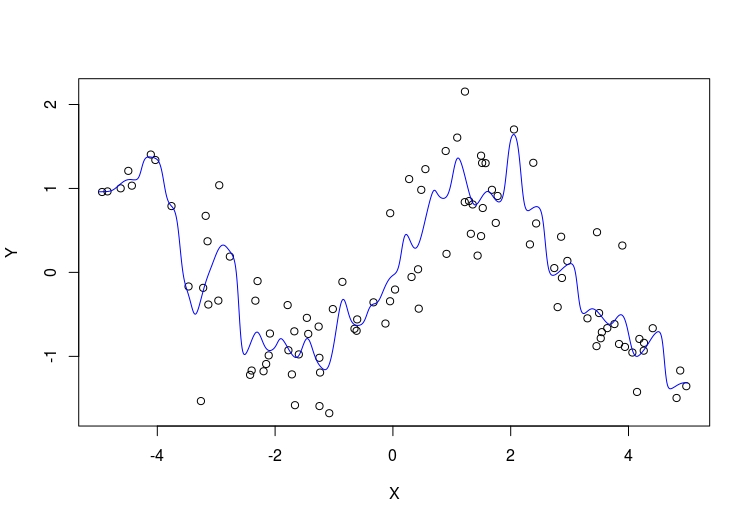
\includegraphics[width = \textwidth]{h01.jpeg}
\caption{Bandwidth \(h = 0.1\)}
\end{figure}


\begin{figure}[h!]
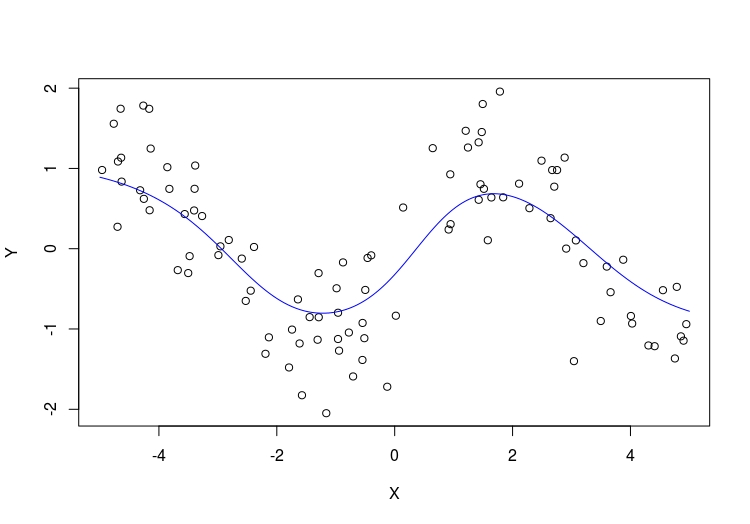
\includegraphics[width = \textwidth]{h1.jpeg}
\caption{Bandwidth \(h = 1\)}
\end{figure}




The bandwidth \(h\) affects the smoothness of the prediction line. With smaller \(h\), more weight is given to neighbor points and the line fluctuates. With larger \(h\), more weight is given to points that are further away, resulting in a smoother line.

\section*{Cross Validation}
\subsection*{B}
For the smooth function, I use \(x^2\); for the wiggly function, I use \(sin(10x)\). `Not so noisy' has a Normal noise of \(0.05\), `noisy' has a Normal noise of \(0.25\). I generate \(100\) points in train and \(100\) points in test. The bandwidth \(h\) is varied from \(0.01\) to \(0.20\). For the smooth function with less noise, the RMSE is stable across different settings of \(h\). But for other cases, using the right \(h\) seems to improve RMSE significantly.
\begin{figure}[h!]
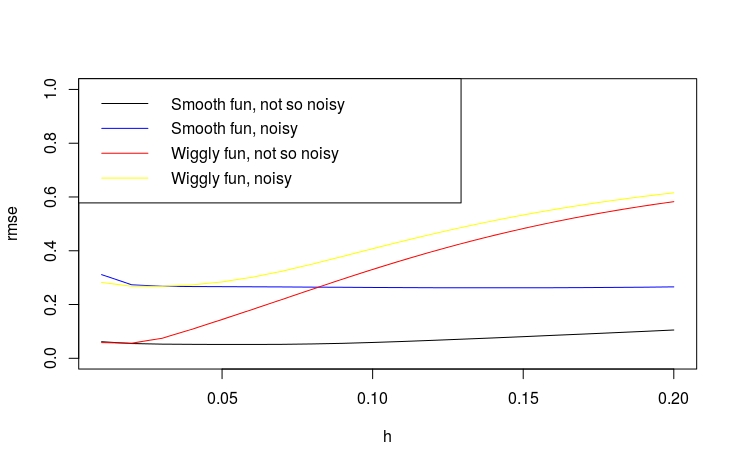
\includegraphics[width = \textwidth]{cv.jpeg}
\caption{Cross Validation}
\end{figure}

\section*{Local polynomial regression}
\subsection*{A}
Let \(R_{x}\) be a \(n \times D\) matrix whose \( (i,j) \) entry is \( (x_i - x)^{j-1}\). We have that
\begin{align*}
g_x(x_i; a) = R_{x,i}^T a
\end{align*}
where \(a\) is the column vector of coefficients of the polynomial \(g\) and \(R_{x,i} \) is the row \(i\) of \(R_{x}\). We want to minimize:

\begin{align*}
&\sum_{i=1}^n w_i \{y_i - g_x(x_i; a)\}^2\\
&= \sum_{i=1}^n w_i \{y_i - R_{x,i}^T a\}^2\\
&= \sum_{i=1}^n \frac{1}{h}K\left(\frac{x_i - x}{h}\right)  \{y_i - R_{x,i}^T a\}^2\\
&= (R_x a - y)^T K_x (R_x a - y)\\
&= a^TR_x^T K_x R_x a  - a^TR_x^T K_x y -  y^T K_x R_x a + y^Ty\\
&= F_x
\end{align*}
where \(K_x\) is the diagonal matrix whose \( (i,i) \) entry is \(\frac{1}{h}K(\frac{x_i - x}{h})\).
We take the derivative and set to zero:
%\begin{align*}
%&\frac{\partial F_x} {\partial a} = \sum_{i=1}^n \frac{1}{h}K\left(\frac{x_i - x}{h}\right) 2 (R_{x,i}^T a - y_i) R_{x,i} = 0\\
%&\implies \sum_{i=1}^n \frac{1}{h}K_{x, i} R_{x,i}^T a R_{x,i} - \sum_{i=1}^n \frac{1}{h}K_{x, i} y_i R_{x,i} = 0 \\
%&\implies \sum_{i=1}^n \frac{1}{h}K_{x, i} R_{x,i,j} a_j R_{x,i,j} - \sum_{i=1}^n \frac{1}{h}K_{x, i} y_i R_{x,i,j} = 0 \hspace{0.5cm} \forall j\\
%&\implies a_j = \frac{\sum_{i=1}^n K_{x, i} y_i R_{x,i,j} } { \sum_{i=1}^n K_{x, i} R_{x,i,j}^2   }
%&\implies K_x R_x R_x a
%\end{align*}

\begin{align*}
\partial F_x / \partial a &= 2 R_x^T K_x R_x a - 2 R_x^T K_x y = 0\\
&\implies a= (R_x^T K_x R_x)^{-1} R_x^T K_x y
\end{align*}

The estimate at \(x\) is \(\hat{f}(x) = a_0 = S_x y\), where
\begin{align*}
S_x = e_1 (R_x^T K_x R_x)^{-1} R_x^T K_x
\end{align*}
\subsection*{B}
For \(D=1\), we have:
\begin{align*}
a &= \begin{pmatrix}
\sum_i K_{x,i} & \sum_i K_{x,i} (x_i - x)\\
\sum_i K_{x,i} (x_i - x) & \sum_i K_{x, i} (x_i - x)^2
\end{pmatrix}^{-1} 
\begin{pmatrix}
K_{x,1} & ... & K_{x,n}\\
K_{x,1}(x_1 - x) & ... & K_{x,n}(x_n - x)\\
\end{pmatrix} y\\
&= \frac{1}{C}\begin{pmatrix}
\sum_i K_{x, i} (x_i - x)^2 & -\sum_i K_{x,i} (x_i - x)\\
-\sum_i K_{x,i} (x_i - x) &  \sum_i K_{x,i}
\end{pmatrix}
\begin{pmatrix}
\sum_i K_{x,i} y_i\\
\sum_i K_{x,i}(x_i - x) y_i\\
\end{pmatrix}\\
&= \frac{1}{C}\begin{pmatrix}
s_2(x) & -s_1(x)\\
-s_1(x) & s_0(x) 
\end{pmatrix}
\end{align*}
where \(C = s_0(x) s_2(x) - s_1(x)^2\). 
We then have:
\begin{align*}
a_0 &= \frac{1}{C} \left[ s_2(x) \sum_i K_{x,i} y_i - s_1(x) \sum_i K_{x,i} (x_i - x) y_i \right]\\
&= \frac{1}{C} \left\lbrace \sum_i K_{x,i}[ s_2(x) - (x_i - x)s_1(x) ] y_i \right\rbrace
\end{align*}
and
\begin{align*}
C &= \sum_i K_{x,i} s_2(x) - \sum_i K_{x,i} (x_i - x) s_1(x)\\
&= \sum_i K_{x,i} \left\lbrace s_2(x) - (x_i - x) s_1(x)\right\rbrace
\end{align*}

Let \( w_i = K_{x,i} \left\lbrace s_2(x) - (x_i - x)s_1(x) \right\rbrace \), we have:
\begin{align*}
\hat{f}(x) = \frac{\sum_i w_i y_i}{w_i}
\end{align*}


\subsection*{C}
The mean is
\begin{align*}
E \hat{f}(x) = E [ S_x y ] = S_x f(X) = \sum_i S_{x,i} f(x_i)
\end{align*}
and the variance is:
\begin{align*}
\mbox{var} \hat{f}(x) &= \mbox{var} [ S_x y ] = \mbox{var} \left( \sum_i S_{x,i} (f(x_i) + e_i) \right)\\
&= \sum_i S_{x,i}^2 \mbox{var}(e_i)\\
&= \sum_i S_{x,i}^2 \sigma^2\\
\end{align*}

\section*{D}

\section*{E}
\textsf{Code: local\_linear.r}

\section*{F}

\begin{figure}
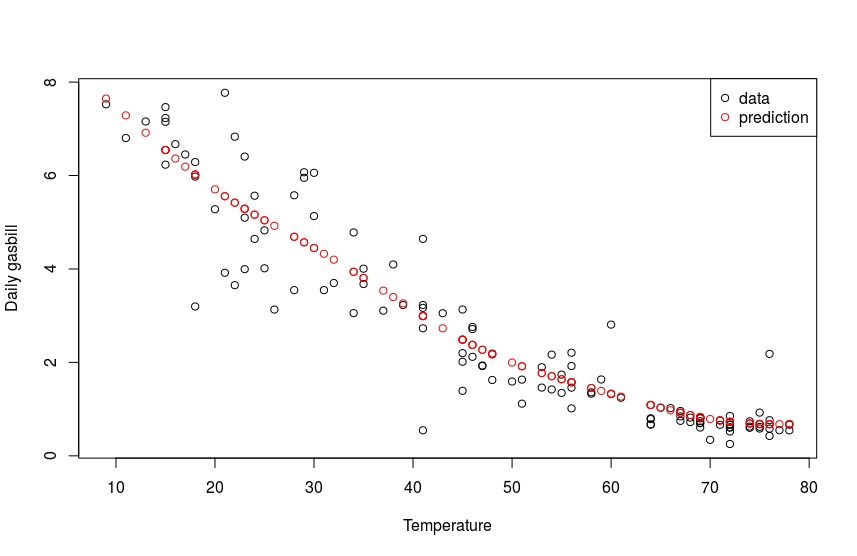
\includegraphics[width=\textwidth]{util_plot.jpeg}
\caption{The data and prediction by local linear estimator}
\label{fig:util}
\end{figure}

\begin{figure}
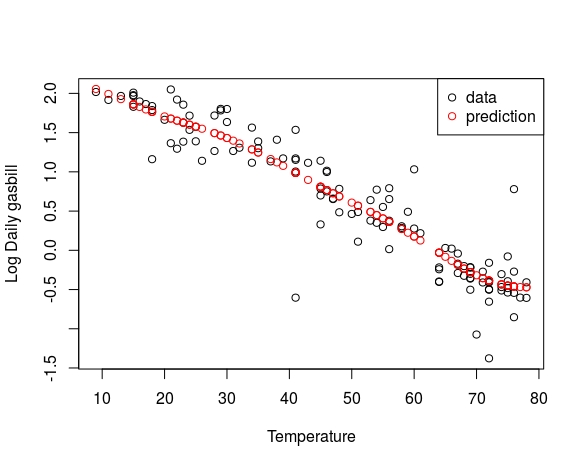
\includegraphics[width=\textwidth]{util_log.jpeg}
\caption{The data and prediction by local linear estimator after a log transformation on the daily gasbill.}
\label{fig:util_log}
\end{figure}

The variance is larger for temperature 20 to 60 and smaller for temperature below 20 or above 60. By taking log on the Daily gasbill, the hemoskedastic assumption is more reasonable.

\section*{G}

\begin{figure}
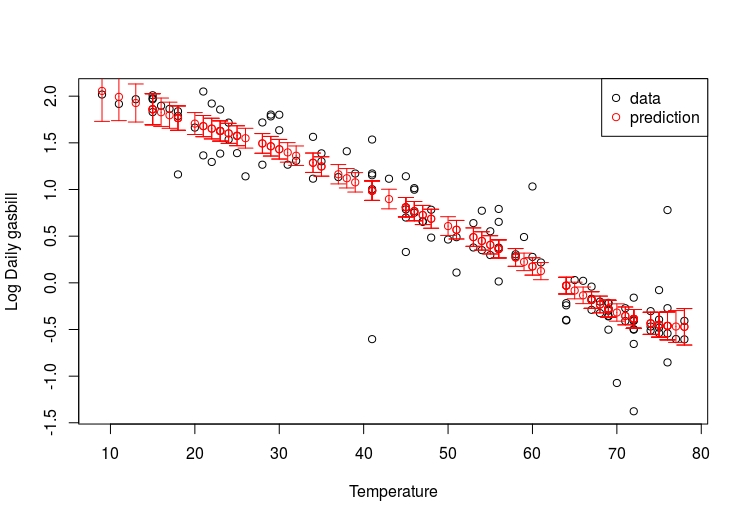
\includegraphics[width=\textwidth]{util_ci.jpeg}
\caption{The data and prediction by local linear estimator after a log transformation on the daily gasbill, with the 95 \% confidence interval.}
\label{fig:util_log}
\end{figure}

\subsection*{Gaussian processes}


\end{document}

